\section{Preliminaries}
\subsection{Notations}
Let $[n]$ be $\{1,2,\dots,n\}$, and let $\I(P)$ denote the
indicator of $P$, i.e., $\I(P)=1$ if $P$ is true, else $0$. 
A labeled graph is represented in a 4-tuple $G = (V, E, \mathcal{L}, l)$, 
where $V$ is a set of vertices, $E \subset V \times V$ is a set of undirected edges, 
$\mathcal{L}$ is a set of labels, 
and $l: V \cup E \rightarrow \mathcal{L}$ is a mapping that assigns each vertex and edge to a label.
We denote as $G \sqsupseteq g$ the
subgraph isomorphism and its negation as $G \not\sqsupseteq g$. 
Thus, a subgraph indicator $\I(G \sqsupseteq g) = 1$ if $G \sqsupseteq g$, otherwise 0.
We also denote the training set of input graphs $G_i \in \Graph$ and output responses $y_i \in \Y$ as
\begin{equation}
  \label{eq:train_data}
  \D = \{(G_1,y_1),(G_2,y_2),\dots,(G_N,y_N)\}, 
\end{equation}
where $\Graph$ is a set of all finite-size, connected, discretely-labeled,
undirected graphs. We denote $\Graph_N = \{G_i\mid i \in [N]\}$, 
and the set of all possible connected subgraphs as $\S_N = \bigcup_{G \in \Graph_N} \{g \mid G \sqsupseteq g\}$.
\begin{definition}{(subgraph isomorphism)}
	Let $G' = (V', E', \mathcal{L}', l')$ and $G = (V, E, \mathcal{L}, l)$, 
	$G'$ is subgraph isomorpic to $G$ iff there exist an injective mapping $\phi: V' \rightarrow V$, 
	s.t., (1) $\forall v \in V, l(v) = l'(\phi(v))$, 
	(2) $\forall (v_{1}, v_{2}) \in E, (\phi(v_{1}), \phi(v_{2})) \in E'$ and
	(3) $l(v_{1}, v_{2}) = l'(\phi(v_{1}), \phi(v_{2}))$.
\end{definition}

\subsection{Search Space for Subgraphs}
\label{sec:subgraphMining}
In supervised learning from graphs, we represent each input graph $G_i \in
\Graph_N$ by the characteristic vector $(\I(G_i \sqsupseteq g) \mid g \in
\S) $ with a set $\S$ of relevant subgraph features. However, since $\S$ is not
explicitly available when the learning phase starts, we need to
simultaneously search and construct $\S$ during the learning process.
In order to define an efficient search space for $\S_N$, i.e., any subgraphs occurring in $\Graph_n$,
the techniques for \textit{frequent subgraph mining} are
useful. Note that any subgraph feature
$g \in \S_N$ can occur multiple times at multiple locations in a single graph,
but $\I(G_i \sqsupseteq g) = 1$.

In the present paper, we use the search space of the gSpan algorithm \cite{Yan:2002},
which performs a depth-first search on the tree-shaped search spaces on $\S_N$,
referred to collectively as an \textit{DFS code tree}, as shown in Figure~\ref{fig:search_tree}.
Each node of the DFS code tree holds a subgraph feature $g'$ that
extends the subgraph feature $g$ at the parent node by one edge, namely, $ g' \sqsupseteq g $.

\begin{figure}[t]
  \centering
  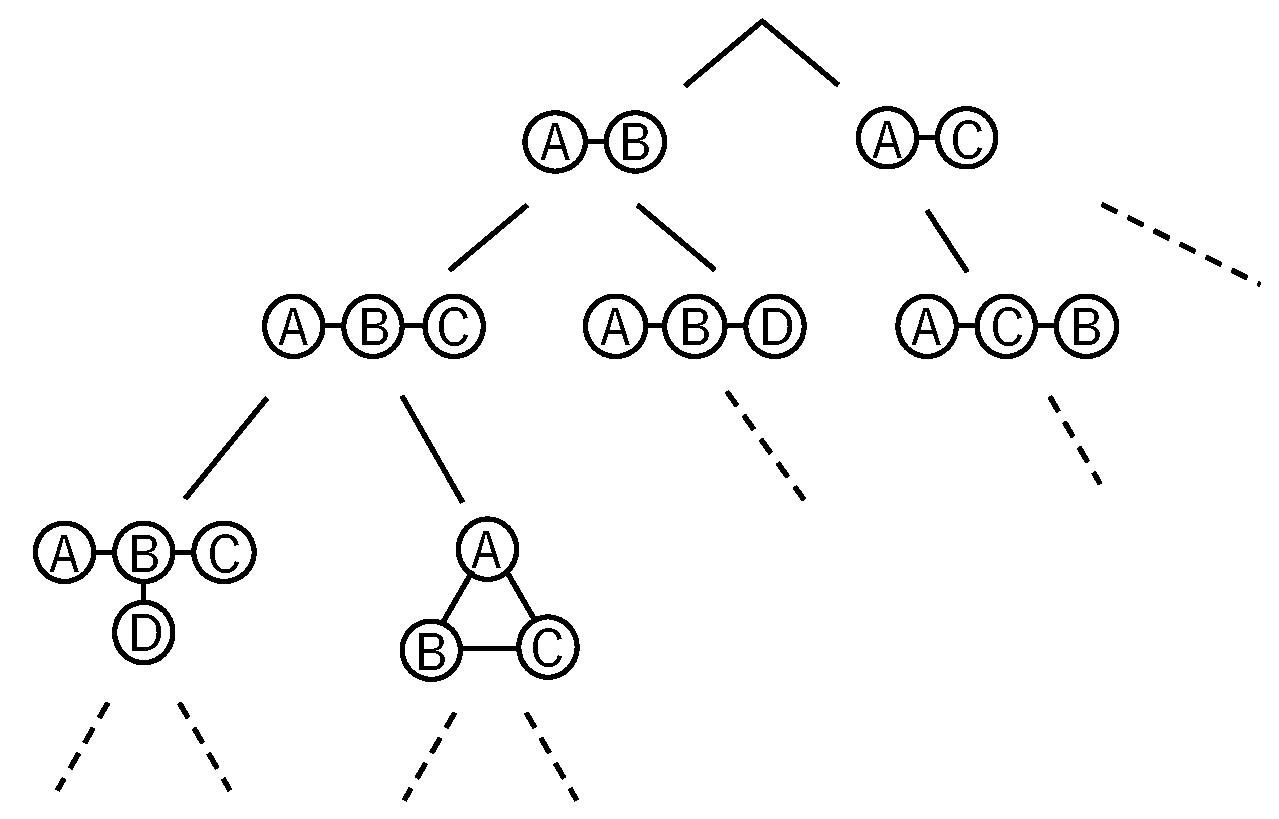
\includegraphics[width=0.5\linewidth]{img/search_tree.eps}
  \caption{DFS code tree}
  \label{fig:search_tree}
\end{figure}

The following \textit{anti-monotone} property of
subgraph isomorphism over the DFS code tree on $\S_N$ can be used to
derive the efficient search-space pruning of the gSpan algorithm:
\begin{equation}
  \label{eq:propSubgraph}
  G_i \not \sqsupseteq g \Rightarrow G_i \not\sqsupseteq g'
  \quad \text{for} \quad
  g' \sqsupseteq g . % period
\end{equation}

\subsection{Discriminative Criteria}
\label{sec:criteria}
Assume we have a two-class problem ($y_{i} \in \{-1, +1\}$).
We evaluate the discriminating degree of each subgraph by the following formulas.
When predicting the graph labels with discrete values, $ClassificatonScore$ $(CScore)$  is used defined as (\ref{eq:score_C}).
\begin{eqnarray}
  \label{eq:score_C}
  CScore(g) = \max \Big[ \sum_{n=1}^{N} y_{n} (2\I(G_{n} \sqsupseteq g) - 1), \sum_{n=1}^{N} y_{n} (2\I(G_{n} \not\sqsupseteq g) -1) \Big]
\end{eqnarray}
This score is the sum of the values that take +1 if the graph label prediction is correct and -1 otherwise.
When predicting the graph labels with real values, $RegressionScore$ $(RScore)$ is used defined as (\ref{eq:score_R}).
\begin{eqnarray}
  \label{eq:score_R}
  RScore(g) &=& \mse(\D_1(g)) + \mse(\D_0(g)) \\
  \mse(\D) &=& \frac{1}{N} \sum_{i \in [N]}
  (y_i - \bar{y})^2, \,\, \bar{y} = \frac{1}{N} \sum_{i \in [N]} y_i. \nonumber
\end{eqnarray}
where MSE is mean squared error, and
$\D_1(g) = \{ (G_i, y_i) \in \D \mid G \sqsupseteq g \} $ and
$\D_0(g) = \{ (G_i, y_i) \in \D \mid G \not\sqsupseteq g \} $.

\begin{comment}
\subsection{Gradient Tree Boosting}
\label{sec:GTB}
Gradient tree boosting (GTB) \cite{friedman2001greedy,
  mason2000boosting} is a general algorithm for supervised learning to
predict a response $y$ from a predictor $\bm{x}$. 
For a given hypothesis space $\H$, the goal is to minimize the empirical
risk $L(f) = N^{-1}\sum_{i \in [N]} \ell(y_i,f(\bm{x}_i))$ of $f \in
\H$, which is the average of a loss function $\ell(y,f(\bm{x}))$ over
the training data $\{(\bm{x}_i, y_i)\}_{i \in[N]}$.

GTB is an additive ensemble model of regression trees
$T_i(\bm{x})$ of the form for fixed-stepsize cases:
\[
f_k(\bm{x}) = T_0 + \eta \sum _{i \in [k]} T_i(\bm{x})
\]
where $T_0$ is the mean of response variables in the training data,
$\eta$ is the stepsize, and $T_i(\bm{x})$ is the $i$-th regression
tree as a base learner. To fit the model to the training data, GTB
performs the following gradient-descent-like iterations as a boosting
procedure:
\begin{eqnarray*}
  f_0(\bm{x}) \leftarrow \arg \min_c \sum_{i \in [N]} \ell(y_i, c), \\
  \quad \text{and} \quad
  f_k(\bm{x}) \leftarrow f_{k-1}(\bm{x}) + \eta \, T_k(\bm{x}),
\end{eqnarray*}
where $T_k(\bm{x})$ is a regression tree to best approximate the values of negative functional
gradient $-\nabla_{f_{k-1}} L(f_{k-1}) $ at $f_{k-1}$ obtained by
fitting a regression tree to the data $\left\{\left(
\bm{x}_i, r_i
\right)\right\}_{i \in [N]}$, where
\begin{equation*}
  r_i =
  -\left[\frac{\partial\, \ell(y_i,
      f(\bm{x}_i))}{\partial
      f(\bm{x}_i)}\right]_{f(\bm{x})=f_{k-1}(\bm{x}_i)}
\end{equation*}
Our experiments focus on binary classification tasks with $y \in
\{-1,+1\}$, and thus we use the logistic loss $\ell(y, \mu) = \log
(1+\exp(-2 y \mu))$. Note that even for classification, GTB must fit
regression trees instead of classification trees in order to approximate
real-valued functions.

The primary hyperparameters of GTB that we consider are
the following three parameters: a max tree-depth $d$, a stepsize $\eta$,
and the number of trees $k$.

\subsection{Regression Trees}
The internal regression-tree fitting is performed by the recursive
partitioning below:
\begin{enumerate}
\item
  Each node in the regression tree receives a subset $\D' \subseteq \D$ from the parent node.
\item
  If a terminal condition is satisfied,
  the node becomes a leaf decision node with a prediction
  value by the average of the response values in $\D'$.
\item
  Otherwise, the node becomes an internal node that tries
  to find the best partition of $\D'$ to $\D_1$ and
  $\D_0 = \D' \setminus \D_1$ that minimizes the total
  sum of squares of residual error $r$:
  \begin{equation*}
    \myargmin{\D_1, \D_0} \bigl[ \tss(\D_1) + \tss(\D_0) \bigr] .
  \end{equation*}
  The subsets $\D_1$ and $\D_0$ are further sent to the child nodes, and
  Step (1) is then recursively applied to each subset at the child nodes.
\end{enumerate}
$\tss$ here is the total sum of squares of residual error $r$:
\begin{equation}
  \label{eq:tss} 
  \tss(\D) = \frac{1}{2} \sum_{i \in [N]}
  (r_i - \bar{r})^2, \,\, \bar{r} = \frac{1}{N} \sum_{i \in [N]}
  r_i.
\end{equation}
\end{comment}
